\documentclass[a4paper]{report}
\usepackage{listings}
\usepackage{enumitem}
\usepackage{mdframed}
\usepackage{graphicx} % Required for the inclusion of images

\title{CEEN 8886: Homework 6}
\date{2017-04-19}
\author{Kelly Boswell}

\begin{document}

\maketitle

\pagenumbering{gobble}

\newpage

\pagenumbering{arabic}

% Problem 1
\section{Problem 1 --- 3G (UMTS) Security}

\subsection{Discuss the new infrastructure requirements in moving from a GSM
            network to UMTS.}

In GSM, the main architectural components are illustrated in Figure \ref{fig:prob1a}.
They are the Mobile Station (MS) which includes the subscriber's SIM card;
the Base Station Subsystem which consists of Base Station
Controller (BSC) and the Base Transceiver Station (BSS); and the Network Subsystem
which consists of the Home Location Register (HLR), the Visitor Location Register
(HLR), the Equipment Identity Register (EIR), the Authentication Centre (AuC), and
the Mobile Service Switching Center (MSC).

In UMTS, the main architectural components are illustrated in Figure \ref{fig:prob1b}
and Figure \ref{fig:prob1c}.  They are the User Equipment (UE) which includes the
users USIM card; the UMTS Terrestrial Radio Access Network (UTRAN) which is composed
of Node Bs used to connect the UE to a the core network via a Radio Network Controller
(RNC); and the core network which consists of the HLR, VLR, EIR, MSC, and AuC but includes
new components to support General Packet Radio Service (GPRS) --- intruduced in 2.5G --- 
for packet-based wireless communications to support TCP/IP communication protocols. These
new components are the Serving GPRS Support Node (SGSN) and the Gateway GPRS Support Node
(GGSN). The core network also consists of a Gateway Mobile Switching Centre (GMSC) used to
interface to external networks.

\begin{figure}
\begin{mdframed}
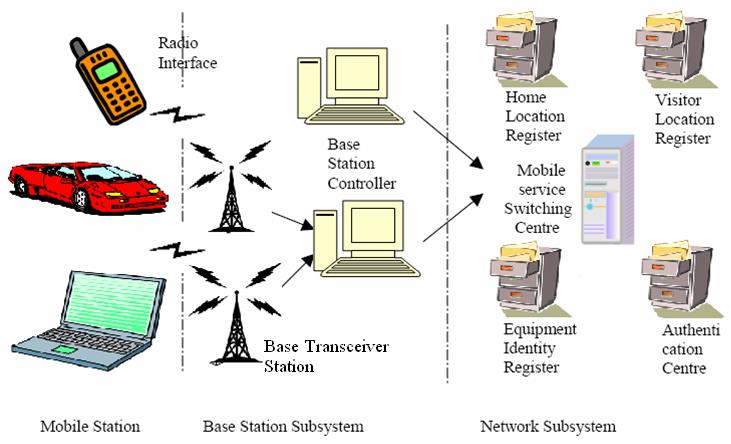
\includegraphics[scale=0.4]{GSM_Architecture.png}
\caption{GSM Architecture}
\label{fig:prob1a}
\end{mdframed}
\end{figure}

\begin{figure}
\begin{mdframed}
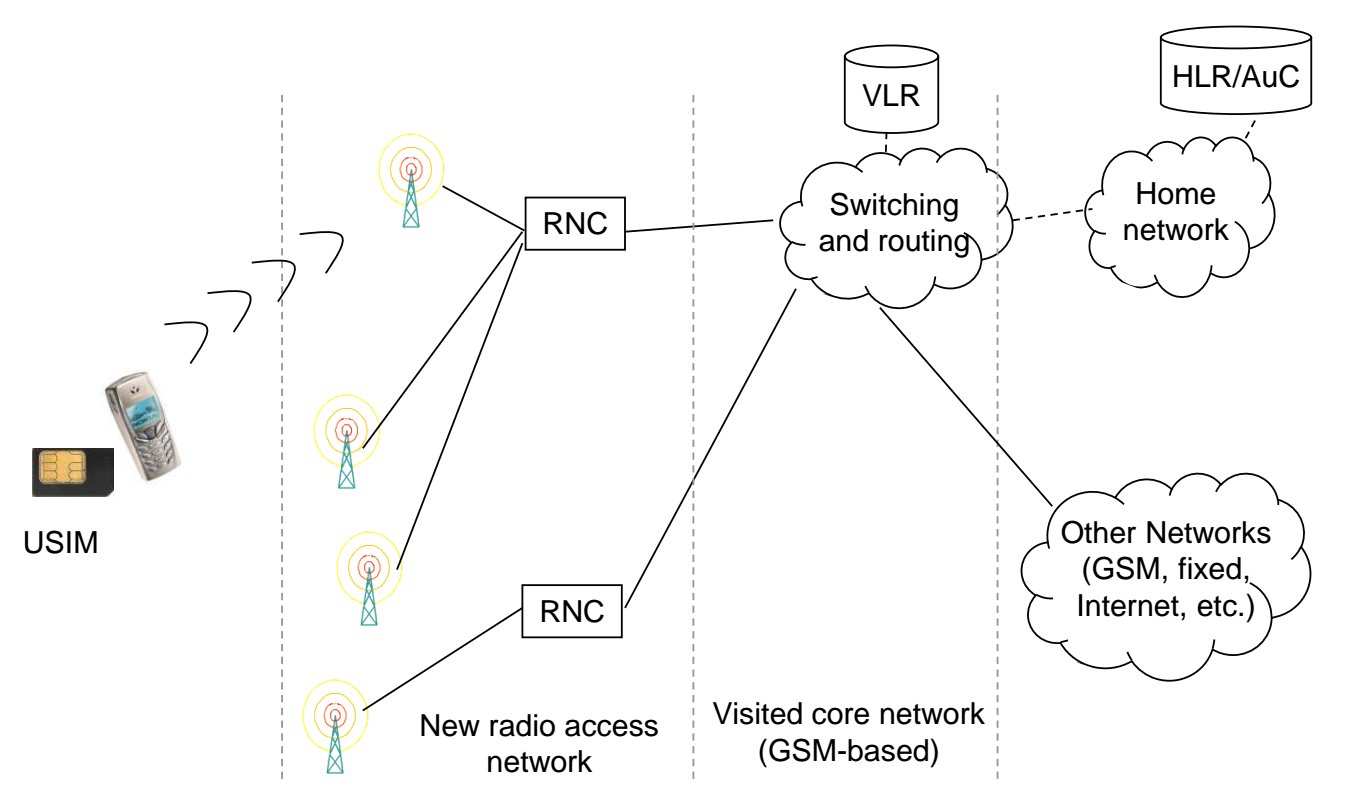
\includegraphics[scale=0.2]{UMTS_Architecture1.jpg}
\caption{3GPP Architecture --- UMTS}
\label{fig:prob1b}
\end{mdframed}
\end{figure}

\begin{figure}
\begin{mdframed}
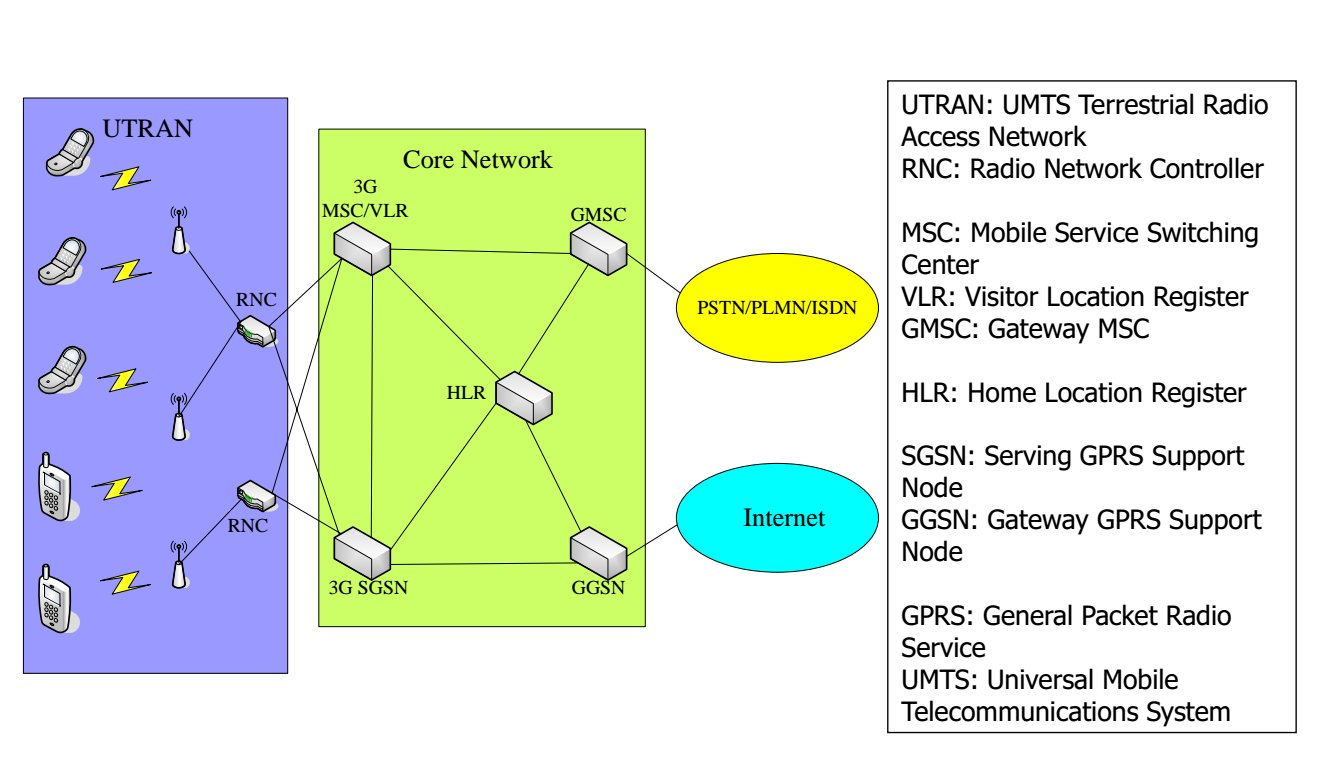
\includegraphics[scale=0.2]{UMTS_Architecture2.jpg}
\caption{3GPP Architecture --- UMTS}
\label{fig:prob1b}
\end{mdframed}
\end{figure}

%Problem 2
\section{Problem 2 --- LTE Security}

\subsection{Illustrate the improvements of LTE security over UMTS security.
            Give detailed explanations.}

%Problem 3
\section{Problem 3 --- IEEE 802.15 for WPAN Security}

Alice is using GSM cellular network to communicate with her friends.

\subsection{What is the hopping rate in Bluetooth and how many bits are
            transmitted in one slot transmission?}


\subsection{Which 802.11 LAN standards will Bluetooth interfere with?}


\subsection{What is the reason for a lower speed/lower power WPAN standard
            such as IEEE 802.15.4?}

\end{document}
